%
% The first command in your LaTeX source must be the \documentclass command.
\documentclass[sigconf]{acmart}
\definecolor{pblue}{rgb}{0.13,0.13,1}
\definecolor{pgreen}{rgb}{0,0.5,0}
\definecolor{pred}{rgb}{0.9,0,0}
\definecolor{pgrey}{rgb}{0.46,0.45,0.48}
\usepackage{tabularx}
\usepackage{listings}

\lstset{language=Java,
 showspaces=false,
 showtabs=false,
 breaklines=true,
 showstringspaces=false,
 breakatwhitespace=true,
 commentstyle=\color{pgreen},
 keywordstyle=\color{pblue},
 stringstyle=\color{pred},
 basicstyle=\ttfamily,
 moredelim=[il][\textcolor{pgrey}]{$$},
 moredelim=[is][\textcolor{pgrey}]{\%\%}{\%\%}
}

\def\code#1{\texttt{#1}}
\long\def\red#1{\textcolor{red}{#1}}

%
% defining the \BibTeX command - from Oren Patashnik's original BibTeX documentation.
\def\BibTeX{{\rm B\kern-.05em{\sc i\kern-.025em b}\kern-.08emT\kern-.1667em\lower.7ex\hbox{E}\kern-.125emX}}

% Rights management information.
% This information is sent to you when you complete the rights form.
% These commands have SAMPLE values in them; it is your responsibility as an author to replace
% the commands and values with those provided to you when you complete the rights form.
%
% These commands are for a PROCEEDINGS abstract or paper.
\copyrightyear{2019}
\acmYear{2019}
\setcopyright{acmlicensed}
\acmConference[LA-WEB]{LA-WEB 2019: 10th Latin American Web Congress}{May 13-14, 2019}{San Francisco, CA, USA}
\acmBooktitle{LA-WEB 2019: 10th Latin American Web Congress. May 13-14, 2019. San Francisco, CA, USA}
\acmPrice{15.00}
\acmDOI{}
\acmISBN{6}

%
% These commands are for a JOURNAL article.
%\setcopyright{acmcopyright}
%\acmJournal{TOG}
%\acmYear{2018}\acmVolume{37}\acmNumber{4}\acmArticle{111}\acmMonth{8}
%\acmDOI{10.1145/1122445.1122456}

%
% Submission ID.
% Use this when submitting an article to a sponsored event. You'll receive a unique submission ID from the organizers
% of the event, and this ID should be used as the parameter to this command.
%\acmSubmissionID{123-A56-BU3}

%
% The majority of ACM publications use numbered citations and references. If you are preparing content for an event
% sponsored by ACM SIGGRAPH, you must use the "author year" style of citations and references. Uncommenting
% the next command will enable that style.
%\citestyle{acmauthoryear}

%
% end of the preamble, start of the body of the document source.
\begin{document}

%
% The "title" command has an optional parameter, allowing the author to define a "short title" to be used in page headers.
\title[After Brazil's GDPR: Authorization in Decentralized Web Applications]{After Brazil's General Data Protection Law: Authorization in Decentralized Web Applications}

%
% The "author" command and its associated commands are used to define the authors and their affiliations.
% Of note is the shared affiliation of the first two authors, and the "authornote" and "authornotemark" commands
% used to denote shared contribution to the research.
\author{Jefferson O. Silva}
\email{silvajo@pucsp.br}
\affiliation{%
 \institution{Pontifical Catholic University of S\~ao Paulo}
 \city{S\~ao Paulo}
 \country{Brazil}
}

\author{Newton Calegari}
\email{newton@nic.br}
\affiliation{%
 \institution{Brazilian Network Information Center - NIC.br}
 \city{S\~ao Paulo}
 \country{Brazil}
}

\author{Eduardo S. Gomes}
\email{egomes@pucsp.br}
\affiliation{%
 \institution{Pontifical Catholic University of S\~ao Paulo}
 \city{S\~ao Paulo}
 \country{Brazil}
}

%
% By default, the full list of authors will be used in the page headers. Often, this list is too long, and will overlap
% other information printed in the page headers. This command allows the author to define a more concise list
% of authors' names for this purpose.
\renewcommand{\shortauthors}{Silva et al.}

%
% The abstract is a short summary of the work to be presented in the article.
\begin{abstract}
Decentralized web applications do not offer fine-grained access controls to users' data, which potentially creates openings for data breaches. For software companies that need to comply with Brazil's  General Data Protection Law (LGPD), data breaches not only might harm application users but also could expose the companies to hefty fines. In this context, engineering fine-grained authorization controls (that comply with the LGPD) to decentralized web application requires creating audit trails, possibly in the source code. Although the literature offers some solutions, they are scattered. We present Esfinge Guardian, an authorization framework that completely separates authorization from other concerns, which increases compliance with the LGPD. We conclude the work with a brief discussion.
\end{abstract}

%
% Keywords. The author(s) should pick words that accurately describe the work being
% presented. Separate the keywords with commas.
\keywords{Access control, Decentralized Web Applications, Frameworks, Guardian, Solid}

%
% This command processes the author and affiliation and title information and builds
% the first part of the formatted document.
\maketitle

\section{Introduction}

With the approval of the Brazilian General Data Protection Law (LGPD, Portuguese acronym) \cite{LGPD18}, several software companies may need to redesign the applications that handle the personal data of Brazilian citizens. The LGPD considers personal any data that directly or indirectly lead to the identification of a user \cite{LGPD18}. Neglecting the LGPD requirements could mean incurring in fines up to 2\% of companies' global revenue \cite{LGPD18}.

The LGPD sets compliance requirements on the companies in charge of making decisions about the data processing (i.e., data controllers) and the companies that process personal data in the name of data controllers (i.e., data processors) \cite{LGPD18}. Besides, the LGPD states that, in some cases, data controllers and data processors may be held liable, especially in cases where data breaches are harmful to users \cite{LGPD18}.

To avoid being classified as either data processors or data controllers (to avoid sanctions), some companies may redesign applications as decentralized web applications. In the context of this research, an application is considered decentralized when it does not hold users' data. Berners-Lee and colleagues \cite{Sambra} proposed a platform called Solid (derived from ``\textbf{So}cial \textbf{li}nked \textbf{d}ata"), which can be described as a set of principles, conventions, and tools for building decentralized web applications. Solid is based on the principle that users should have full ownership of their data, which are stored in Web-accessible personal online datastores (pods) \cite{Sambra}. Pods are independent of web applications. For obtaining services, users need to authorize web applications to access their pods explicitly, by classifying web applications as trusted.

Using Solid alone leaves users solely responsible for controlling access to protected resources, which may not be enough to comply with the LGPD. The LGPD requirement of data governance (see Art. 50, Par. 2 in \cite{LGPD18}) states that, among other things, companies should establish adequate policies to protect users' data. Nevertheless, in Solid web applications, a user would not have the means to prevent unauthorized access to their data, after classifying a web application as trusted. For example, a hospital web application may have a sensitive operation that reads personal data from patient's pods that should be accessible only by designated doctors. A violation of this access control policy would configure a data breach, in which case the hospital might still be held liable. Also, the liability risk might create the need for audits, in which case it would be necessary that the hospital demonstrated that it possesses appropriate controls, possibly directly in source code.

This context indicates that it is necessary to engineer fine-grained authorization controls, without loosing the simplicity required in auditing the source code. Thus, we establish the following research question (RQ).

\vspace{0.15cm}
\noindent \textbf{RQ: How to design fine-grained authorization controls to decentralized web applications that comply with the LGPD requirement of data governance?}
\vspace{0.15cm}

The answer to our RQ may help companies to increase compliance with the LGPD by employing several software engineering techniques, which are implemented in Esfinge Guardian. With this paper, we contribute to the literature in at least two ways. First, by showing that the decentralization of a web application may not be enough for companies to avoid liability issues. Second, by pointing the need for more research on how the use of Esfinge Guardian (and others) could increase compliance with the LGPD (and other regulations).

This work is organized as follows. In Chapter 2, we offer some background. In Chapter 3, we present Esfinge Guardian. In Chapter 4, we offer a case example. In Chapter 5, we present some related works. We conclude with a brief discussion in Chapter 6.


\section{Background}
In this section, we offer some background for the understanding of the research problem domain.

\subsection{Brazil's General Data Protection Law}

The Brazil's General Data Protection Law (LGPD) is based on the General Data Protection Regulation (GDPR),\footnote{\url{http://data.consilium.europa.eu/doc/document/ST-9565-2015-INIT/en/pdf}} which aims at protecting the personal data of EU individuals. In total, around 120 countries adopt comprehensive privacy laws and regulations to protect personal data held by private and public bodies \cite{Banisar2011}. The LGPD applies to any individual or legal entity (public or private) with personal data processing activities that: are carried out in Brazil; offer or supply goods or services in Brazil or relate to individuals located in Brazil, and; involve personal data collected in Brazil.

\subsection{Decentralized Solid Web Applications}

Traditional web applications (e.g., Facebook, CRMs, and hospital applications) rely on private APIs, exclusive access control mechanisms, and dedicated data storage sytems. Because users cannot move personal data to other platforms, these web applications become ``data silos." We refer to these web applications as centralized \cite{VanKleek2012}.

Solid is a platform that supports decentralized web applications, by relying on open standards and semantic web technologies \cite{Bern09}. In the Solid platform, applications run in a browser or as mobile applications, while users data are stored in pods \cite{Bern06}. Although pods can be stored locally, they typically are stored in dedicated servers, which manage data according to the Linked Data Platform recommendation, enabling it to manipulate data items through HTTP requests \cite{LDP}. Solid servers are application-agnostic and can deal with both structured and unstructured data. Structured data is represented using RDF, a Semantic Web standard \cite{Bern06,Hollenbach2009}. Application development based on Solid platform supports portability and interoperability, so applications can be seen as an interface that works with distributed data in multiple pod server implementations.

Identity in the Solid context is based on WebID, which allows agents (e.g., a person, an organization) to create their identities using global unique identifiers - HTTP URIs \cite{Sambra}. A WebID is an open and decentralized identification mechanism being developed by a W3C community group.\footnote{\url{https://www.w3.org/community/webid/}}

In a decentralized web application model, resources created by an application and can be updated by a different one without prior agreement between the applications. It is possible because the applications are interfaces to access data stored in multiple locations, such as in pods.

\subsection{Authorization in Solid}

Access control is typically split into two distinct procedures: authentication, and authorization. While authentication is concerned with determining whether an agent (e.g., user, group) is whom it claims to be, authorization is responsible for verifying if the agent is allowed to access a protected resource (e.g., document) or operation (e.g., read, write, append). In this research, we focus on authorization.

Solid uses the Web Access Control (WAC) specification for authorizing the access to protected resources. According to the specification, WAC has the following key features:

\begin{enumerate}
\item The resources are identified by URLs and can refer to any web documents or resources;
\item It is declarative -- access control policies are written in regular web documents;
\item Users and groups are also identified by URLs (WebIDs);
\item It is cross-domain -- all of its components, such as resources, agent WebIDs, and even the documents containing the access control policies, can potentially reside on separate domains;
\end{enumerate}


\begin{lstlisting}[escapeinside=||,caption={Example WAC Document}, captionpos=b,label={lst:individual-permission}]
 |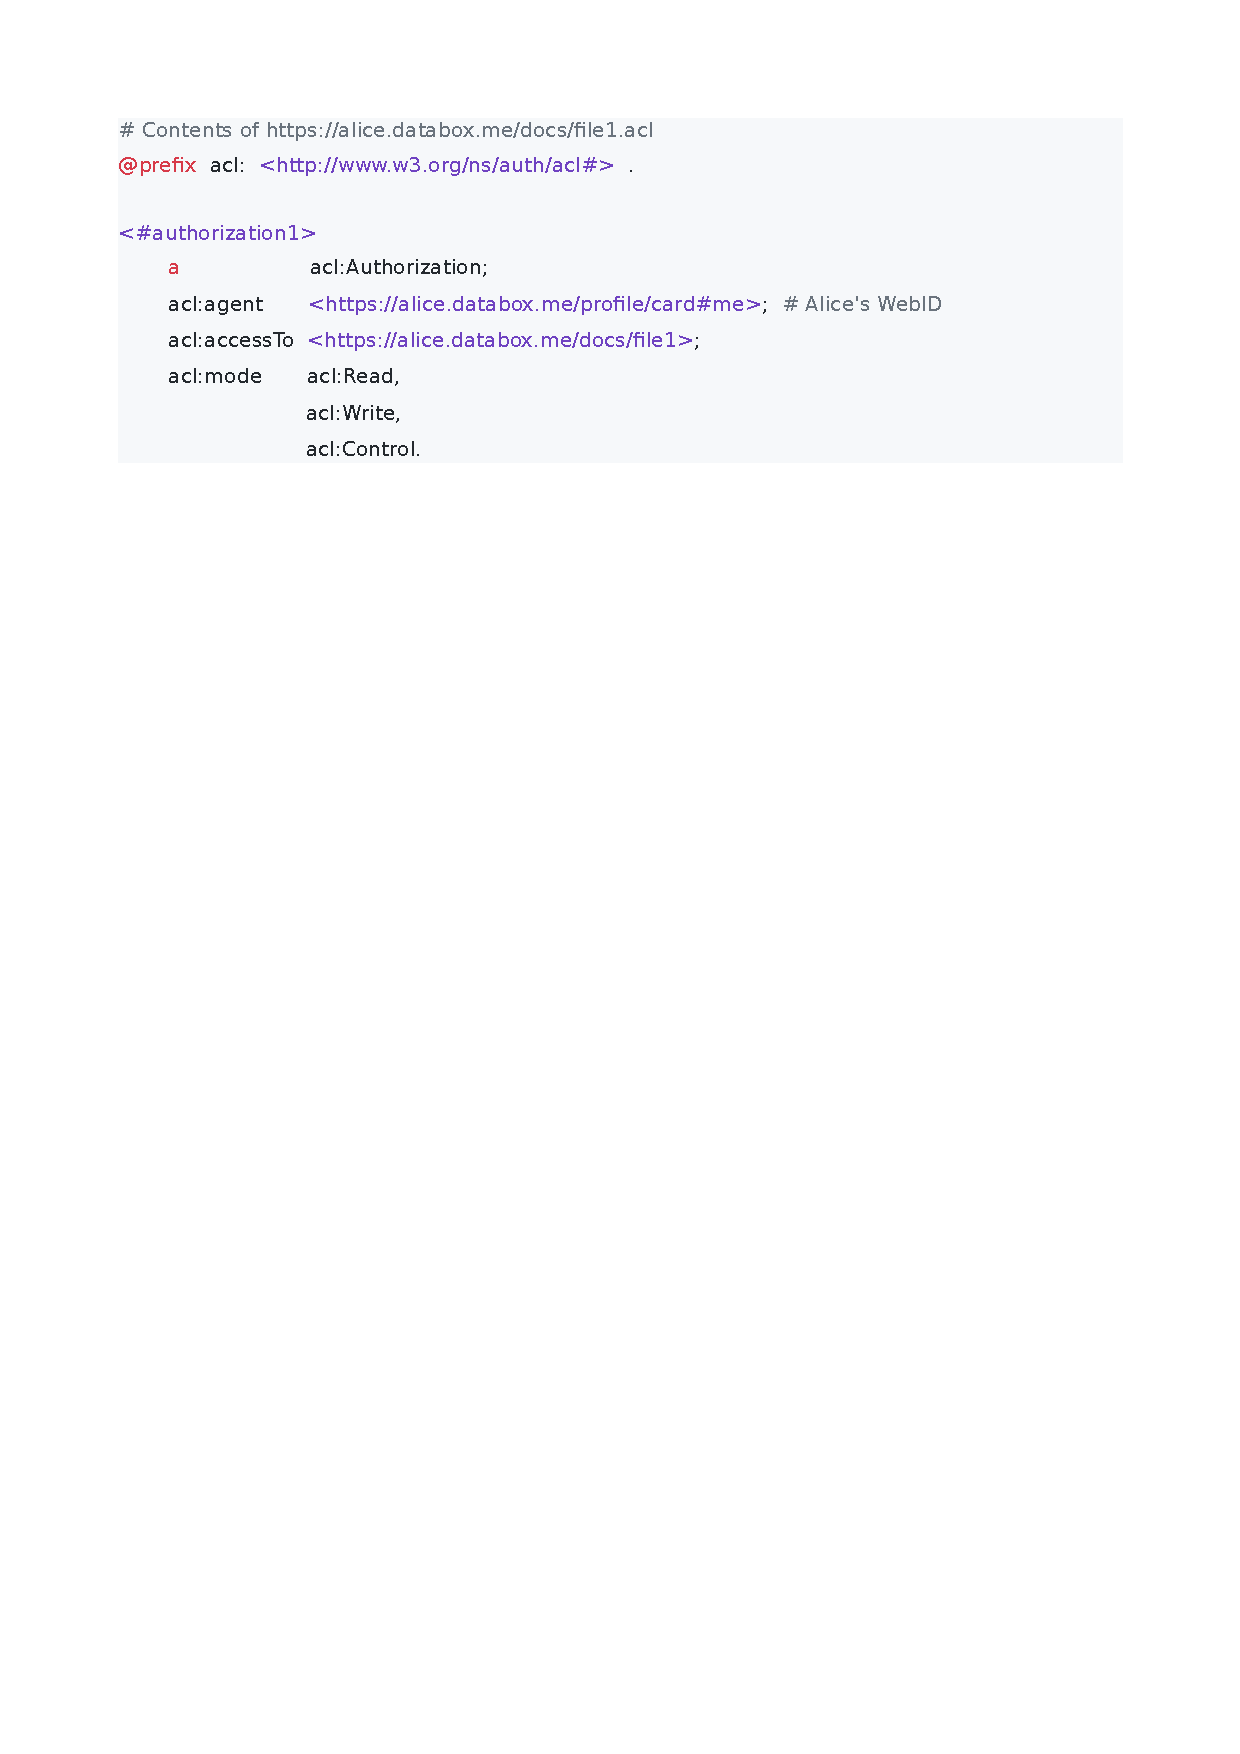
\includegraphics[trim=2cm 21.9cm 4.7cm 2cm, clip, scale=0.57]{pdf/alice-permission}|
\end{lstlisting}

Listing \ref{lst:individual-permission} shows an example of a WAC document that specifies that Alice (as identified by her WebID \code{https://alice.\\databox.me/profile/card\#me}) has full access (read, write, and control) to one of her web resources, located at \code{https://\\alice.databox.me/docs/file1}.

Similarly, it is possible to give access to a group of agents using the \code{acl:agentGroup} predicate \cite{ONTO}. A group is a collection of members (or WebIDs) that needs to be specified in a different file. Moreover, it is possible to give access to all agents (public access) or yet to all authenticated agents. Besides, it is also possible to classify web applications as trusted. Furthermore, not every document needs its own individual access control list file. Rather, it is possible to authorize a container, which is a web location that contain multiple resources.
As mentioned, for controlling the access to the data in their pods, users need to specify WAC documents. The set of authorization modes that WAC access control systems offer does not allow the specification of fine-grained authorizations, required for decentralized web applications that needed to comply with the LGPD.

%%%%%%%%%%%%%%%%%%%%%%%%%%%%%%%%%%%%%%%%%%%%%%
%%%%% NEW SECTION
%%%%%%%%%%%%%%%%%%%%%%%%%%%%%%%%%%%%%%%%%%%%%%
\section{Esfinge Guardian}

In this section, we present the Esfinge Guardian\footnote{\url{https://github.com/EsfingeFramework/guardian}} framework. Essentially, the Esfinge Guardian's role is to intercept calls to protected operations. Figure \ref{fig:interception-mechanism} depicts a hypothetical interception. As an example, consider a protected operation \verb|debit()|, which should only be executed by the account owner. Esfinge Guardian would intercept the call to \verb|debit()|, and decide if the caller is authorized to perform the operation.

\begin{figure}
 \centering
 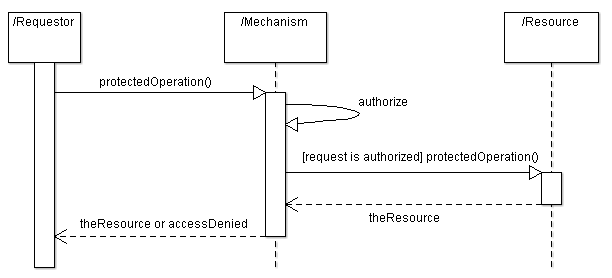
\includegraphics[scale=0.5]{img/interception-mechanism.png}
 \caption{A conceptualization of the interception mechanism (Silva et al. \cite{Silva2013})}
 \label{fig:interception-mechanism}
\end{figure}

Additionally, Figure \ref{fig:guardian-in-decentralized-webapp} depicts Esfinge Guardian in a hypothetical web decentralized hospital application. As depicted, Esfinge Guardian contains the authorization logic that will only allow authorized HTTP requests to a patient's pods. Besides, while Esfinge Guardian is independent of decentralized web applications (and consequentially of Solid), employing the framework may help these applications increase compliance with LGPD. We stress that although Figure \ref{fig:guardian-in-decentralized-webapp} depicts Esfinge Guardian authorizing access to pods based on roles, it can authorize in finer-grained levels.

Esfinge Guardian is composed of eight elements (see Guerra et al. \cite{Guerra2015} and Silva et al.\cite{Silva2013} for in-depth explanations). Figure \ref{fig:class-diagram} depicts the relationship between the elements in UML.

\vspace{0.8mm} \noindent \verb|AuthorizationContext|. It is the central entity that holds all the information required for an authorization, which includes the data for the subject, resource, and environment. That means all other entities should provide \verb|AuthorizationContext| with enough information for authorization to occur.

\vspace{0.8mm} \noindent \verb|GuardianInterceptor|.
Ideally, the user must be able to indicate what operations should be protected and be oblivious of all other things. A request to a protected operation must be intercepted transparently, not directly called. \verb|GuardianInterceptor| is the entity responsible for abstracting the different existing interception technologies such as aspect-orientation, CGLib, and dynamic proxy.

\begin{figure}
  \centering
  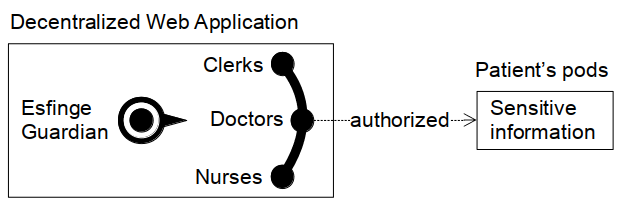
\includegraphics[scale=0.5]{img/guardian-in-decentralized-webapp.png}
  \caption{Esfinge Guardian representation in a decentralized web application}
  \label{fig:guardian-in-decentralized-webapp}
\end{figure}

\vspace{0.8mm} \noindent \verb|Invoker|.
The original request to the protected operation on the resource is intercepted; therefore the mechanism must be in charge of replicating the request to the resource if the access is granted. \verb|Invoker| is an entity with the ability to mimic the operation performed by the subject on a protected resource. In the Esfinge Guardian framework, this element can execute methods; however, it is important to note that it is just one of the possibilities since the architectural model is general.

One additional feature is that \verb|Invoker| is responsible for determining when the authorization logic is performed. In many cases, enforcing the authorization logic only makes sense after the protected operation is performed. For instance, consider the case when the operation retrieves a collection, and the authorization rule requires iterating it in order to verify if the subject can indeed access all of its items. In this manner, there should be a way for configuring the precise moment that the authorization should take place.

\begin{figure*}
 \centering
 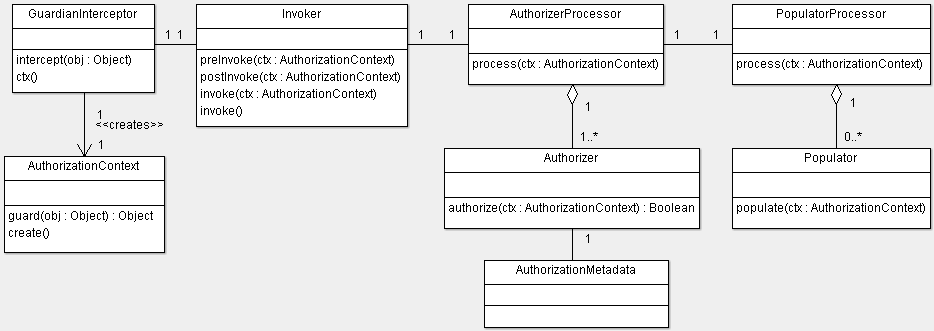
\includegraphics[scale=0.4]{img/guardian-class-diagram.png}
 \caption{The Esfinge Guardian Class Diagram (Silva et al.\cite{Silva2013})}
 \label{fig:class-diagram}
\end{figure*}

\vspace{0.8mm} \noindent \verb|Populator|.
It is the entity that contains the data extraction logic for authorization. Information for authorization can be anywhere such as databases, files, shared variables, user session, arguments, and the Internet. For this reason, \verb|Populator| is an entity that knows how to obtain information from all these places.
There can be zero or more \verb|Populators| in the application; each one specialized in obtaining a different type of information from a different place.

\vspace{0.8mm} \noindent \verb|PopulatorProcessor|.
The entity that gathers and executes all defined \verb|Populators| in the application.

\vspace{0.8mm} \noindent \verb|Authorizer|. This is entity that implements the logic of the access control policy and may use information stored in \verb|AuthorizationContext| if necessary. There must be at least one \verb|Authorizer|. Every \verb|Authorizer| respond in the form of a ``yes" or ``no;" however, it must be possible to include other response types such as ``Indeterminate."

\vspace{0.8mm} \noindent \verb|AuthorizerProcessor|.
It is the entity that contains the combining algorithm for all the \verb|Authorizers| defined in the application.

\vspace{0.8mm} \noindent \verb|AuthorizationMetada|.
This is an entity that indicates which resources---or their operations---must be intercepted by the authorization mechanism. A requirement is that this element must be of metadata type so that it can be used declaratively. Esfinge Guardian uses Java annotations as the implementation of this element; however, it can be considered a general marking element that is independent of a specific technology.





\section{Related Works}

This research combines topics usually addressed separately. We are not aware of any research that addresses the LGPD from a software engineering perspective. Alternatively, some researchers studied approaches that map GDPR principles to software design. For example, Danezis et al. \cite{Ed2014} provided an inventory of privacy design strategies and technical building blocks of various degrees of maturity from research and development. Koops and Leenes \cite{Koops2014} discussed whether the GDPR Privacy-by-Design principle entails hard-coding privacy requirements into applications. On decentralized web applications, Berners-Lee \cite{Bern09} introduced the concept of decentralized application architectures. Smith et al. \cite{Smith2012} introduced a functional decentralized application called WebBox, while Dodson et al. \cite{Dodson2012} presented Musubi, a disintermediated interactive social feeds application for mobile devices. Concerning metadata-based frameworks such as Esfinge Guardian, Guerra et al. \cite{Guerra2010} investigated metadata usage in existing frameworks and documented recurrent solutions as architectural patterns.

\section{Discussion and Conclusion}

The LGPD requires companies to adopt a comprehensive data governance approach, including data profiling, data lineage, data masking, test-data management, and data archives. Also, specialized professionals are required to design and handle personal data. In this work, we show how Esfinge Guardian can be used to manage authorizations in decentralized web applications to increase compliance with the LGPD's data governance requirements. Besides the examples we offered, Esfinge Guardian could be used to anonymize personal data, filtering information that could lead to users identification.

%
% The acknowledgments section is defined using the "acks" environment (and NOT an unnumbered section). This ensures
% the proper identification of the section in the article metadata, and the consistent spelling of the heading.
\begin{acks}
To the Brazilian Network Information Center (NIC.br) and the Web Technologies Study Center (Ceweb.br) for supporting this research.
\end{acks}

%
% The next two lines define the bibliography style to be used, and the bibliography file.
\bibliographystyle{ACM-Reference-Format}
\bibliography{laweb19}


\end{document}
